%\documentstyle[10pt,twoside]{article}
%\documentstyle[twoside]{article}
\documentclass[twoside]{article}
\setlength{\oddsidemargin}{0.25 in}
\setlength{\evensidemargin}{-0.25 in}
\setlength{\topmargin}{-0.6 in}
\setlength{\textwidth}{6.5 in}
\setlength{\textheight}{8.5 in}
\setlength{\headsep}{0.75 in}
\setlength{\parindent}{0 in}
\setlength{\parskip}{0.1 in}

\usepackage{graphicx}
\usepackage{url}

%
% The following commands sets up the lecnum (lecture number)
% counter and make various numbering schemes work relative
% to the lecture number.
%
\newcounter{lecnum}
\renewcommand{\thepage}{\thelecnum-\arabic{page}}
\renewcommand{\thesection}{\thelecnum.\arabic{section}}
\renewcommand{\theequation}{\thelecnum.\arabic{equation}}
\renewcommand{\thefigure}{\thelecnum.\arabic{figure}}
\renewcommand{\thetable}{\thelecnum.\arabic{table}}
\newcommand{\dnl}{\mbox{}\par}

%
% The following macro is used to generate the header.
%
\newcommand{\lecture}[4]{
   \pagestyle{myheadings}
   \thispagestyle{plain}
   \newpage
   \setcounter{lecnum}{#1}
   \setcounter{page}{1}
   \noindent
   \begin{center}
   \framebox{
      \vbox{\vspace{2mm}
    \hbox to 6.28in { {\bf CMPSCI~677~~~Operating Systems
                        \hfill Spring 2018} }
       \vspace{4mm}
       \hbox to 6.28in { {\Large \hfill Lecture #1: #2  \hfill} }
       \vspace{2mm}
       \hbox to 6.28in { {\it Lecturer: #3 \hfill Scribe: #4} }
      \vspace{2mm}}
   }
   \end{center}
   \markboth{Lecture #1: #2}{Lecture #1: #2}
   \vspace*{4mm}
}

%
% Convention for citations is authors' initials followed by the year.
% For example, to cite a paper by Leighton and Maggs you would type
% \cite{LM89}, and to cite a paper by Strassen you would type \cite{S69}.
% (To avoid bibliography problems, for now we redefine the \cite command.)
%
\renewcommand{\cite}[1]{[#1]}

% \input{epsf}

%Use this command for a figure; it puts a figure in wherever you want it.
%usage: \fig{NUMBER}{FIGURE-SIZE}{CAPTION}{FILENAME}
\newcommand{\fig}[4]{
            %\vspace{0.2 in}
            \centerline{\includegraphics[scale=#2]{#4}}
            \begin{center}
            Figure \thelecnum.#1:~#3
            \end{center}
    }

% Use these for theorems, lemmas, proofs, etc.
\newtheorem{theorem}{Theorem}[lecnum]
\newtheorem{lemma}[theorem]{Lemma}
\newtheorem{proposition}[theorem]{Proposition}
\newtheorem{claim}[theorem]{Claim}
\newtheorem{corollary}[theorem]{Corollary}
\newtheorem{definition}[theorem]{Definition}
\newenvironment{proof}{{\bf Proof:}}{\hfill\rule{2mm}{2mm}}

% Some useful equation alignment commands, borrowed from TeX
\makeatletter
\def\eqalign#1{\,\vcenter{\openup\jot\m@th
  \ialign{\strut\hfil$\displaystyle{##}$&$\displaystyle{{}##}$\hfil
      \crcr#1\crcr}}\,}
\def\eqalignno#1{\displ@y \tabskip\@centering
  \halign to\displaywidth{\hfil$\displaystyle{##}$\tabskip\z@skip
    &$\displaystyle{{}##}$\hfil\tabskip\@centering
    &\llap{$##$}\tabskip\z@skip\crcr
    #1\crcr}}
\def\leqalignno#1{\displ@y \tabskip\@centering
  \halign to\displaywidth{\hfil$\displaystyle{##}$\tabskip\z@skip
    &$\displaystyle{{}##}$\hfil\tabskip\@centering
    &\kern-\displaywidth\rlap{$##$}\tabskip\displaywidth\crcr
    #1\crcr}}
\makeatother

% **** IF YOU WANT TO DEFINE ADDITIONAL MACROS FOR YOURSELF, PUT THEM HERE:



% Some general latex examples and examples making use of the
% macros follow.

\begin{document}

%FILL IN THE RIGHT INFO.
%\lecture{**LECTURE-NUMBER**}{**DATE**}{**LECTURER**}{**SCRIBE**}
\lecture{9}{February 21}{Prashant Shenoy}{\textbf{Ankita Mehta}}

\section{Lightweight RPC (LRPC)}
Lightweight RPCs are the special case of RPCs where calling process and the called process are on the same machine.\\
When client and server both are on the same machine, following are the things which can make it better over the traditional RPC:
\begin{enumerate}
\item No need for the marshalling here.
\item We can get rid of explicit message passing completely. Rather shared memory is used as a way of communication.
\item Stub can use the run-time flag can be used to decide whether to use TCP/IP or shared memory.
\item No XDR is required.
\end{enumerate}

Steps of execution of LRPC:
\begin{enumerate}
\item Arguments of the calling process are pushed on the stack,
\item Trap to kernel is send,
\item After sending trap to kernel, it either constructs an explicit shared memory region and put the arguments there or take the page from stack and simply turn it into shared page,
\item Client thread executed procedure (OS upcall),
\item Then the thread traps to the kernel upon completion of the work,
\item Kernel again changes back the address space and returns control to client,
\end{enumerate}

\textbf{Note:} RPCs are called "doors" in SUN-OS (Solaris).

\section{Other RPC models}

Traditional RPC uses Synchronous/blocked RPC, where the client gets blocked making an RPC call and gets resumed only after getting result from the called process. There are three other RPC models described below:

\begin{figure}[h]
\begin{center}
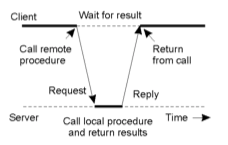
\includegraphics[scale=0.8]{images/trad_RPC}
\caption{Traditional RPC}
\end{center}
\end{figure}

\subsection{Asynchronous RPC}

In Asynchronous or non-blocking RPC call, the client is not blocked after making an RPC call. Rather it sends the request and waits for an acknowledgement from the called process and after getting the acceptance, it resumes the execution.

\begin{figure}[h]
\begin{center}
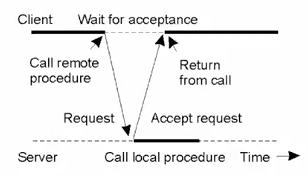
\includegraphics[scale=0.8]{images/async_RPC}
\caption{Asynchronous RPC}
\end{center}
\end{figure}

\subsection{Deferred synchronous RPC}

This is just a variant of Non-blocking RPC as in this Client and server interact through two asynchronous RPCs. Here the server send the replies to the client by making another asynchronous RPC call.

\begin{figure}[h]
\begin{center}
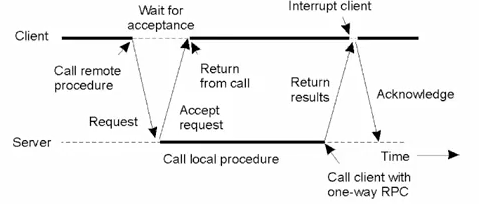
\includegraphics[scale=0.8]{images/deferred_sync_RPC}
\caption{Deferred Synchronous RPC}
\end{center}
\end{figure}

\subsection{One-way RPC}

It is also a form of asynchronous RPC where the waits for an acknowledgment from the server. But in this one-way RPC call, the client doesn't even for an acknowledgment from the server. It starts its execution just after sending a request.
This model has one disadvantage that it doesn't guarantee the reliability as the client doesn't know whether the request reaches the server or not.

\section{Remote Method Invocation (RMI)}
RMIs are RPCs in Object Oriented Programming Mode i.e., they can call the methods of the objects (instances of a class) which are residing on a remote machine. Here the objects hide the face that they are remote.The functional is called just like it is called on a local machine. For eg: obj.foo() , where obj is the object and foo is its public function. Some important facts about RMIs: 
\begin{enumerate}
\item There is equivalent separation between interface and the implementation as the interface is residing on the client machine whereas the implementation is on server machine.
\item It supports system-wide object references i.e parameters can be passed as object references here ( which is not possible in normal RPC)
\end{enumerate}

Figure \ref{distributed_obj} is showing an RMI call between the distributed objects. Just like a normal RPC, here also there is no need to setup socket connections separately by the programmer. Client stub is called the proxy and the server stub is called the skeleton and the instantiated object is one which is grayed in figure.

Now, when the client invokes the remote method, the RMI call comes to the \textit{stub} (Proxy), it realizes that the object is on the remote machine. So it sets up the TCP/IP connection and the marshalled invocation is sent accross the network. Then the server unpacks the message, perform the actions and send the marshalled reply back to the client.

\begin{figure}[h]
\begin{center}
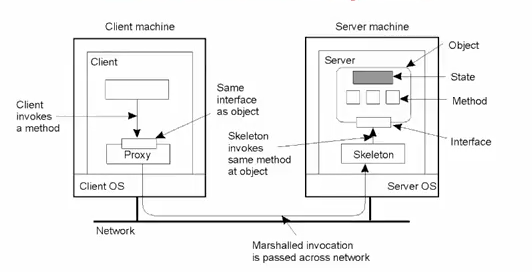
\includegraphics[scale=0.7]{images/RMI}
\caption{Distributed Objects}
\label{distributed_obj}
\end{center}
\end{figure}

\subsection{Proxies and Skeletons : Client and Server Stub}

\begin{itemize}

\item Working of Proxy : Client stub

\begin{enumerate}
	\item Maintains server ID, endpoints, object ID.
	\item Sets up and tears down connection with the server
	\item Serializes (Marshalling) the local object parameters.
\end{enumerate}

\item Working of Skeleton : Server stub

It deserializes and passes parameters to server and sends results back to the proxy.

\end{itemize}

\subsection{Binding a Client to an Object}

Binding can be of two types : implicit and explicit. Section (a) of Figure \ref{binding_client} shows an implicit binding, which is using just the global references and it is figured out on the run-time that it is a remote call (by the client stub). In section (b), explicit binding is shown, which is using both global and local references. Here, the client is explicitly calling a bind function before invoking the methods.  Main difference between both the methods is written in Line 4 of the section (b), where the programmer has written an explicit call to the bind function.

\begin{figure}[h]
\begin{center}
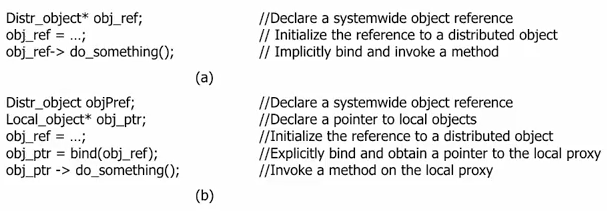
\includegraphics[scale=0.6]{images/binding_client}
\caption{Implicit and Explicit Binding of Clients to an Object}
\label{binding_client}
\end{center}
\end{figure}

\subsection{Parameter Passing}

RMIs are less restrictive than RPCs as it supports system-wide object references. Here, Passing a reference to an object means passing a pointer to its memory address over the network. In Java, local objects are passed by value, and remote objects are passed by reference. Figure \ref{passing_param} shows an RMI call from Machine A(client) to the Machine C (server - called function is present on this machine) where Object O1 is passed as a local variable and Object O2 is passed as a reference variable. Machine C will maintain a copy of Object O1 and access Object O2 by dereferencing the pointer. \\
\textbf{Note:} Since a copy of Object O1 is passed to the Machine C, so if any changes are made to its private variable, then it won't be reflected in the Machine C. Also, Concurrency and synchronization needs to be taken care of.

\begin{figure}[h]
\begin{center}
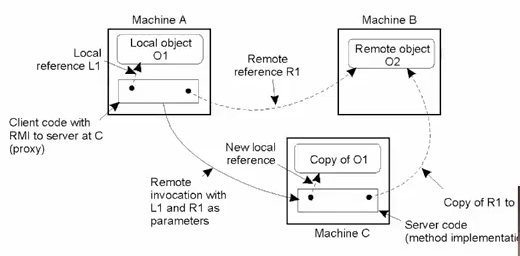
\includegraphics[scale=0.6]{images/param_passing}
\caption{Parameter Passing : RMI}
\label{passing_param}
\end{center}
\end{figure}

\subsection{DCE Distributed-Object Model}

Below are some examples of how invocation of remote objects works across many systems. Clients making requests to server using RMI calls. In section (a) of Figure \ref{Distributed}, every request instantiates a new thread and new local copy of the object (private to that thread). Here after sending the reply, thread is deleted. In section (b), all requests are operated on the same object.There are multiple threads and they all are calling methods of the same object. So all threads are using the state of the object. If one thread make the changes, they will be visible to other threads. Here also, concurrency and synchronisation needs to be taken care of.
\begin{figure}[h]
\begin{center}
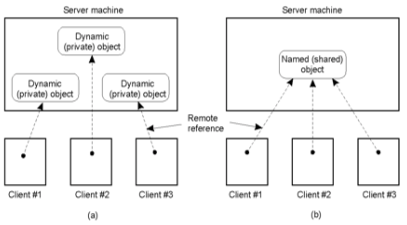
\includegraphics[scale=0.6]{images/DCE}
\caption{Distributed Object Models}
\label{Distributed}
\end{center}
\end{figure}

\section{Java RMI}

\begin{itemize}

	\item Server:
	\begin{itemize}
	\item The server defines the interface and implements the interface methods. The server program creates a server object and registers object with "remote object" registry (Directory service).
	\end{itemize}
	\item Client:
	\begin{itemize}
	\item It looks up the server in remote object registry, and then make the normal call to the remote methods.
	\end{itemize}
	\item Java tools:
		\begin{itemize}
		\item \texttt{rmiregistry}: Server-side name server
		\item \texttt{rmic}: Uses server interface to create client and server stub. it is a RMI Compiler, which creates an autogenerated code for stubs.
		\end{itemize}

\end{itemize}


\subsection{Java RMI and Synchronisation}
Java supports monitors , which are the synchronised objects. The same method can be used for remote method Invocation which allows concurrent requests to come in and synchronisation them. So for synchronisation, lock has to applied on the object which is distributed amongst the clients. How to implement the notion of the distributed lock? 
\begin{enumerate}
\item Lock at the server :  Here, clients will make requests to the server, where they will contend for the lock and will be blocked (waiting for the lock).
\item Lock at the client (proxy) collectively : They will have some protocol which decides which client will get the lock and rest others will be blocked (waiting for the lock)
\end{enumerate}

\textbf{Note:} Java uses proxies for blocking : which means client side blocking.

\section{Message-oriented Transient Communication}

Here in Figure \ref{socket_communication}, It has been shown how the client and sever can communicate using vanilla network sockets. It is the most primitive form of network communication that uses TCP/IP or UDP/IP. Here, firstly a socket is created and then it is used to connect the client to a server and then use that network for communication between them. \\
Steps taken by the client and server to establish socket networking:
\begin{enumerate}
\item Create a new socket
\item Bind the socket or assign the port number to it which will allow the socket to listen on that port number.
\item Then the server is ready to accept the network packets and will wait for the client to send the packet.
\item Then the client will make a socket call (to construct a socket) and make a connection to the server using the server's IP address and the port number to which it is listening.
\item Then they will be connected and they will use the read-write or send-receive call.
\item Once done Close the socket connection
\end{enumerate}

\textbf{Note:} Socket communication is blocking/synchronous in nature.

\begin{figure}[h]
	\begin{center}
		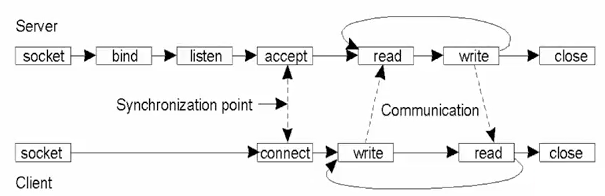
\includegraphics[scale=0.7]{images/sockets}
		\caption{Socket communication}
		\label{socket_communication}
	\end{center}
\end{figure}

One example of sockets are the Berkeley sockets(Figure \ref{BSD} since they appeared in Berkeley System Distribution UNIX (BSD UNIX), but now they are part of the POSIX standards. 

\begin{figure}[h]
	\begin{center}
		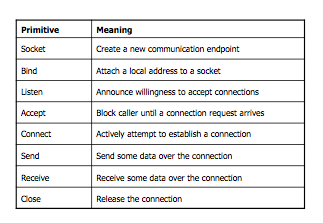
\includegraphics[scale=0.7]{images/BSD}
		\caption{Berkeley Primitives}
		\label{BSD}
	\end{center}
\end{figure}


\section{Message-Passing Interface (MPI)}

MPI(Message Passing Interface) is a library/middleware designed for parallel or distributed applications which need to do a lot of IPC. Since traditional TCP/IP imposes a high overhead, so there is a need of an application which provides control over how data is send and receive that normal socket programming doesn't allow. MPI allows many types of send and receive whereas in socket programming, there is only one type of send-receive.

\begin{figure}[h]
\begin{center}
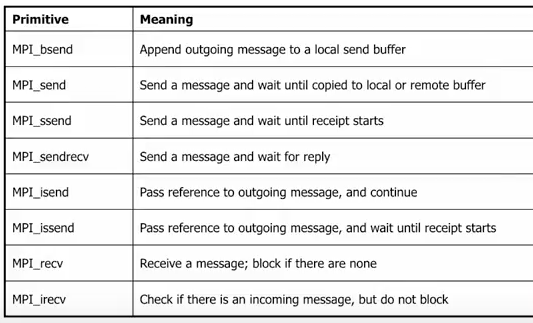
\includegraphics[scale=0.5]{images/MPI_Primitives}
\caption{MPI Primitives}
\label{mpi_primitives}
\end{center}
\end{figure}

Figure \ref{mpi_primitives} shows a list of MPI primitives. MPI has six different variants of send and 2 variants of receive.  Here are some of them explained below:
\begin{enumerate}
\item \textbf{MPI\_bsend}: Message placed in local buffer (but not sent out) and then return. (Non-blocking communication)
\item \textbf{MPI\_send}: Wait until message gets to remote machine and waits for acknowledgement.
\item \textbf{MPI\_sscend}: Wait until receipt starts. It is like Asynchronous/Non-blocking RPC call.
\item \textbf{MPI\_sendrecv}: After sending message, it will wait for reply. Just like in Berkeley primitives (socket programming) or Synchronous RPC.
\item \textbf{MPI\_isend}: Send a pointer to buffer, not even send a copy.
\item \textbf{MPI\_recv}: It is a blocking receive.
\item \textbf{MPI\_irecv}: It is a Asynchronous/Non-blocking receive.
\end{enumerate}

%Descriptive list
%\begin{description}
%  \item[DOS] : small explanation
%  \item[NOS] : small explanation
%  \item[Middleware] : small explanation
%  \item[Multiprocessor OS] : small explanation
%  \item[Multicomputer OS]: small explanation
%\end{description}

\end{document}
